\chapter{Non-Inverting Amplifier}
\section{Proof Of Concept}
\begin{figure}[tp]
	\centering
	\begin{subfigure}{0.4\textwidth}
		\centering
		%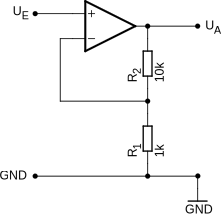
\includegraphics[width=.9\linewidth]{./img/schem-noninv.pdf}
		\caption{Basic Non-Inverting Amplifier with Gain 11}
		\label{schem:non_inv}
	\end{subfigure}
	\begin{subfigure}{0.4\textwidth}
		\centering
		%\includegraphics[width=.9\linewidth]{./img/non_inv_curve.pdf}
		\caption{Non-Inverting Amplifier:\newline $V_\text{pp,in}=\SI{55.2}{\milli\volt}, V_\text{pp,out}=\SI{600}{\milli\volt}$}
		\label{subfig:non_inv_curve}
	\end{subfigure}
	\caption{Schematic And Voltage Curves Of a Non-Inverting Setup}
\end{figure}
\autoref{schem:non_inv} shows the schematic of a non-inverting OpAmp.
As both inputs of the OpAmp virtually are at the same potential, the amplification can be calculated easily by using the voltage divider formula (as seen in \autoref{eq:bias_volt})
\begin{align*}
	V_\text{e}&=V_\text{a}\cdot\frac{R_1}{R_1+R_2} \\
	\Leftrightarrow\ A &=1+\frac{R_2}{R_1}.
\end{align*}
To examine the validity of this relation, the circuit is built and the output voltage is measured as a function of the input voltage.
The resulting curves are shown in \autoref{subfig:non_inv_curve}.
\begin{table}[b!]
	\centering
	\caption{Input, output voltages $V_\text{pp,in/out}$ and resulting voltage amplification $A$ at $f=\SI{1}{\kilo\hertz}$}
	\label{tab:non_inv_vals}
	\begin{tabular}{SSS}
		\toprule
		{$V_\text{pp,in}$ in $\si{\milli\volt}$}&	{$V_\text{pp,out}$ in $\si{\volt}$}&	{$A$}\\
		\midrule
		\num{55.2}	&	\num{0.608}	&	\num{11.01}\\
		\num{352}	&	\num{3.96}	&	\num{11.25}\\
		\bottomrule
	\end{tabular}
\end{table}
In both measurements, the gain is $\approx 11$, which confirms the expectations.

\section{Input And Output Impedances}
